
%\begin{centering}
%    \Huge{\textbf{Curry Stir Fry}}
    
%\end{centering}
%\vspace{8mm}
%\textbf{PRELIMINARIES:}




\bigskip

\bigskip

\begin{multicols}{2}
\textbf{Ingredients}
\begin{itemize}
\item 2 bell peppers \quad (62 kCal/ 2 gP/ 0 gF/ 12 gC)

\item 1 yellow or white onion \quad (50 kCal/ 1 gP/ 0gF/ 10 gC)
\item 1 can sliced chestnuts \quad (65 kCal/ 1 gP/ 0 gF/ 15 gC)
\item 1 can bamboo shoots \quad (40 kCal/ 1 gP/ 0gF/ 9 gC)
\item 1 can bean sprouts \quad (35 kCal/ 4gP/ 0 gF/ 7 gC)
\item 2 boxes of golden curry (medium hot or hot) \newline (900 kCal/ 10 gP/ 45 gF/ 100 gC)
\item 2 lbs broccoli florets \quad (308 kCal/ 26 gP/ 4 gF/ 60 gC)
\item 3 tbsp. olive oil \quad (360 kCal/ 0gP/ 42gF/ 0 gC)
\item 2 lbs chicken breast \quad (750 kCal/ 246 gP/62 gF/ 0 gC)
\item 2 cups jasmine rice \quad (1280 kCal/ 24gP/ 0gF/ 288gC)
\item a shit load of garlic ($\sim$6 cloves) \quad  (80 kCal)
\item 1 tbsp. red pepper flakes
\item $\frac{1}{2}$ tsp. ground ginger
\item 1 tsp. curry powder 
\item 2 tsp. salt

\end{itemize}


\columnbreak
\textbf{Procedure:}
\medskip


\begin{enumerate}
\item 
Begin by cutting the broccoli into bite-sized florets into the pot, dicing the onion and cutting the bell peppers into bite-sized pieces. Set onion and bell pepper aside. 

\item In a large pot or wok, add broccoli, bamboo shoots, and watered chestnuts. Drizzle 2 tbsp of oil on top and sautee on medium heat until broccoli starts to darken.


\medskip
\item Cube the chicken breast and in a separate pan, cook in 1 tbsp of olive oil until done. Cook the rice in a separate pan and leave covered.
\medskip

\item Add the onion, bell pepper, and garlic to the broccoli and continue cooking until broccoli is softened and onions are translucent. Add the golden curry bars and continue cooking for a couple minutes making sure that the curry bricks do not stick to the bottom of the pan.
\newline 

 \item Once the bars have softened, add water and stir until sauce is thick but the curry bars have dissolved. Add bean sprouts and bring to a boil stirring well and making sure nothing is sticking to the bottom. Season with red pepper flakes, ground ginger, and extra curry powder to taste. Serve over rice.  
\end{enumerate}
\begin{centering}
\begin{table}[H]
  \begin{center}
    \caption{Macro totals}
    \label{tab:table1}
    \begin{tabular}{c|c|c|c} % <-- Alignments: 1st column left, 2nd middle and 3rd right, with vertical lines in between
      \textbf{Calories} & \textbf{Protein} & \textbf{Fat} & \textbf{Carbs}\\
      \hline
      4,000 kCal & 315 g & 153 g & 501 g\\
    \end{tabular}
  \end{center}
\end{table}
\end{centering}
\end{multicols}



\begin{center}
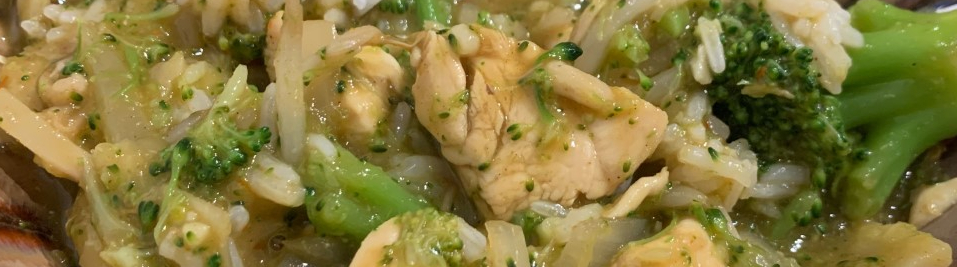
\includegraphics[scale=0.55]{Chicken Recipes/Curry Stir Fry/Curry Stir Fry.jpg}
\end{center}
%I suppose pictures could go here


